% ===========================================================================
% Scaffold-ChunGS 本科毕业论文
% 学校模板匹配：请根据 Word 模板的格式要求调整下方参数
% 编译：xelatex -> biber -> xelatex -> xelatex
% ===========================================================================
\documentclass[zihao=-4,a4paper,oneside,openany]{ctexbook}

% ---------------------------------------------------------------------------
% 页面布局（请根据 Word 模板的页边距要求修改）
% ---------------------------------------------------------------------------
\usepackage[top=2.54cm, bottom=2.54cm, left=3.17cm, right=3.17cm]{geometry}

% ---------------------------------------------------------------------------
% 字体与中文支持
% ---------------------------------------------------------------------------
\usepackage{fontspec}
\setmainfont{Times New Roman}
\setCJKmainfont{SimSun}[AutoFakeBold=2.5]

% ---------------------------------------------------------------------------
% 常用宏包
% ---------------------------------------------------------------------------
\usepackage{amsmath,amssymb}          % 数学公式
\usepackage{algorithm}                % 伪代码
\usepackage{algpseudocode}
\usepackage{graphicx}                 % 图片
\usepackage{subcaption}               % 子图
\usepackage{booktabs}                 % 三线表
\usepackage{longtable}                % 长表格
\usepackage{array}                    % 表格列格式
\usepackage{multirow}                 % 合并行
\usepackage{listings}                 % 代码块
\usepackage{xcolor}                   % 颜色
\usepackage{hyperref}                 % 超链接
\usepackage{enumitem}                 % 列表格式

% ---------------------------------------------------------------------------
% 参考文献 (GB/T 7714-2015 中国标准)
% ---------------------------------------------------------------------------
\usepackage[backend=biber,style=gb7714-2015,sorting=nyt]{biblatex}
\addbibresource{thesis.bib}

% ---------------------------------------------------------------------------
% 代码高亮样式
% ---------------------------------------------------------------------------
\definecolor{codebg}{RGB}{245,245,245}
\definecolor{codeframe}{RGB}{200,200,200}
\lstset{
    backgroundcolor=\color{codebg},
    basicstyle=\small\ttfamily,
    breaklines=true,
    frame=single,
    rulecolor=\color{codeframe},
    numbers=left,
    numberstyle=\tiny\color{gray},
    tabsize=2,
    language=C++,
    showstringspaces=false,
    captionpos=b,
}

% ---------------------------------------------------------------------------
% 超链接样式
% ---------------------------------------------------------------------------
\hypersetup{
    colorlinks=true,
    linkcolor=black,
    citecolor=black,
    urlcolor=blue,
}

% ---------------------------------------------------------------------------
% 自定义命令
% ---------------------------------------------------------------------------
\newcommand{\ScaffoldChunGS}{\textsc{Scaffold-ChunGS}\xspace}
\newcommand{\schun}{\texttt{.schun}\xspace}

\begin{document}

% ===========================================================================
% 封面（按学校 Word 模板填写）
% ===========================================================================
\begin{titlepage}
\centering

\vspace*{4cm}

{\huge\bfseries 基于锚点压缩与分块外存管理的\\[6pt] 大场景3D高斯SLAM系统设计与实现}

\vspace{2cm}

{\Large \textbf{Scaffold-ChunGS: Compressed 3D Gaussian SLAM\\[4pt] with Chunk-Based Out-of-Core Memory Management}}

\vspace{3cm}

\begin{tabular}{rl}
\textbf{学\quad 院：} & \underline{\hspace{3cm}} \\[8pt]
\textbf{专\quad 业：} & \underline{\hspace{3cm}} \\[8pt]
\textbf{姓\quad 名：} & \underline{\hspace{3cm}} \\[8pt]
\textbf{学\quad 号：} & \underline{\hspace{3cm}} \\[8pt]
\textbf{指导教师：} & \underline{\hspace{3cm}} \\[8pt]
\end{tabular}

\vspace{2cm}
{\large \today}

\end{titlepage}

% ===========================================================================
% 中文摘要
% ===========================================================================
\chapter*{摘\quad 要}
\addcontentsline{toc}{chapter}{摘要}

3D高斯泼溅（3D Gaussian Splatting, 3DGS）近年来在三维场景重建与实时渲染领域取得了突破性进展，并逐步被引入视觉SLAM系统中。然而，标准3DGS面临两大瓶颈：（1）每个高斯椭球体需存储59个独立参数，导致稠密重建时GPU显存占用巨大；（2）场景规模受限于显存容量，无法处理大范围环境。

针对上述问题，本文设计并实现了一个融合锚点压缩场景表示与分块外存管理的统一3D高斯SLAM系统——\ScaffoldChunGS。系统的主要工作包括：

\textbf{（1）锚点压缩场景表示。}采用Scaffold-GS的体素化锚点表示，以稀疏锚点（体素中心 + 特征向量）替代密集高斯，通过三个视角条件MLP（不透明度、协方差、颜色）在渲染时动态解码子高斯参数。该方案将单高斯存储开销从约240字节压缩至约28字节（以每锚点5个子高斯计），压缩比约8.6倍。

\textbf{（2）分块外存管理。}将场景按空间划分为固定大小的块（Chunk），设计LRU淘汰策略将非活跃块换出至磁盘，仅保留可见区域在GPU显存中。定义了自包含的\schun 二进制块格式，完整保存锚点参数与Adam优化器状态，支持训练的暂停与恢复。

\textbf{（3）统一C++/LibTorch系统框架。}在C++17/CUDA环境下构建完整的SLAM系统，包含两级视锥剔除、多目标损失函数（L1+SSIM+深度+各向同性正则化）、层级化锚点生长与剪枝、以及基于损失加权的关键帧采样等模块。

实验在合成球面场景上验证了系统的功能完整性，并分析了锚点压缩率、块I/O性能及各模块的消融效果。结果表明，\ScaffoldChunGS 在理论上可将单GPU显存可支撑的场景规模从约30M高斯扩展至无上限（受限于磁盘容量），同时保持与标准3DGS可比的渲染质量。

\vspace{1cm}
\noindent\textbf{关键词：} 3D高斯泼溅；视觉SLAM；场景压缩；外存管理；锚点表示

% ===========================================================================
% 英文摘要
% ===========================================================================
\chapter*{Abstract}
\addcontentsline{toc}{chapter}{Abstract}

3D Gaussian Splatting (3DGS) has achieved breakthroughs in 3D scene reconstruction and real-time rendering, and has been increasingly integrated into visual SLAM systems. However, standard 3DGS faces two major bottlenecks: (1) each Gaussian ellipsoid requires 59 independent parameters, leading to prohibitive GPU memory consumption in dense reconstruction; (2) the scene scale is limited by GPU memory capacity, preventing handling of large-scale environments.

To address these issues, this thesis designs and implements \ScaffoldChunGS—a unified 3D Gaussian SLAM system that combines anchor-based compressed scene representation with chunk-based out-of-core memory management. The main contributions include:

\textbf{(1) Anchor-based compressed scene representation.} Adopting Scaffold-GS's voxelized anchor representation, sparse anchors (voxel centers + feature vectors) replace dense Gaussians. Three view-conditioned MLPs (opacity, covariance, color) dynamically decode child Gaussian parameters at render time. This scheme compresses per-Gaussian storage from approximately 240 bytes to approximately 28 bytes (for 5 child Gaussians per anchor), achieving a compression ratio of approximately 8.6×.

\textbf{(2) Chunk-based out-of-core memory management.} The scene is spatially partitioned into fixed-size chunks. An LRU eviction policy swaps inactive chunks to disk, retaining only the visible region in GPU memory. A self-contained \schun binary chunk format stores all anchor parameters and Adam optimizer states, supporting training suspension and resumption.

\textbf{(3) Unified C++/LibTorch system framework.} A complete SLAM system is built in a C++17/CUDA environment, featuring two-level frustum culling, multi-objective loss functions (L1+SSIM+depth+isotropic regularization), hierarchical anchor growing and pruning, and loss-weighted keyframe sampling.

Experiments on a synthetic sphere scene validate the system's functional completeness and analyze anchor compression ratio, chunk I/O performance, and ablation effects of each module. Results show that \ScaffoldChunGS can theoretically extend per-GPU-memory scene capacity from approximately 30M Gaussians to unlimited (bounded only by disk capacity), while maintaining rendering quality comparable to standard 3DGS.

\vspace{1cm}
\noindent\textbf{Keywords:} 3D Gaussian Splatting; Visual SLAM; Scene Compression; Out-of-Core Memory; Anchor-Based Representation

% ===========================================================================
% 目录
% ===========================================================================
\tableofcontents
\listoffigures
\listoftables

% ===========================================================================
% 正文
% ===========================================================================
% ===========================================================================
% 第一章 绪论
% ===========================================================================
\chapter{绪论}

\section{研究背景与意义}

三维场景重建是计算机视觉与机器人领域的核心问题之一，其目标是从传感器数据中恢复环境的几何结构与外观信息。该技术在增强现实（AR/VR）、自动驾驶、机器人导航、数字孪生以及文化遗产数字化保护等领域具有广泛的应用前景。

传统三维重建方法主要包括基于体素（Volumetric）的TSDF（Truncated Signed Distance Function）融合\cite{curless1996volumetric}和基于点云的结构从运动（Structure from Motion, SfM）\cite{snavely2006photo}。TSDF方法受限于固定分辨率网格，无法同时捕捉大范围场景与精细细节；点云方法虽灵活但缺乏完整的外观信息，难以生成逼真的可视化效果。

2020年，神经辐射场（Neural Radiance Fields, NeRF）\cite{mildenhall2020nerf}的提出标志着三维重建进入神经网络时代。NeRF通过MLP隐式表达场景的密度与颜色场，配合体渲染实现照片级新视角合成。然而，NeRF的体渲染需沿每条射线密集采样，导致训练与推理速度极慢（单场景训练需数小时），难以满足实时SLAM需求。

2023年，3D高斯泼溅（3D Gaussian Splatting, 3DGS）\cite{kerbl20233dgaussians}横空出世，以显式的3D高斯椭球体取代隐式MLP表示，通过可微光栅化实现快速渲染与梯度反向传播。3DGS将训练时间从数小时缩短至数十分钟，渲染帧率达实时级别（$\ge$30 FPS），迅速成为三维视觉领域的研究热点\cite{chen2024surgey}。

然而，标准3DGS在面对大规模场景时面临严峻的\textbf{内存瓶颈}：

\begin{enumerate}[label=(\arabic*),leftmargin=2em]
    \item \textbf{单高斯存储开销大。}每个高斯椭球体需存储位置$\mathbf{x}\in\mathbb{R}^3$、颜色（球谐系数，最高48维）、不透明度$\alpha\in\mathbb{R}$、协方差矩阵（尺度$\mathbf{s}\in\mathbb{R}^3$ + 旋转四元数$\mathbf{q}\in\mathbb{R}^4$），合计约59个浮点参数（$\sim$240 bytes/高斯）。对于中等规模的室内场景，高斯数量即可达到数百万量级，单场景显存占用轻易突破8 GB。
    \item \textbf{场景规模受限。}所有高斯参数及其Adam优化器状态需常驻GPU显存，场景范围严格受限于显存容量。在室外大规模建图中，这一约束尤为严重。
\end{enumerate}

针对上述问题，学术界在两条技术路线上取得了重要进展：

\begin{itemize}
    \item \textbf{锚点压缩表示（Scaffold-GS）\cite{lu2024scaffoldgs}}：以稀疏的体素化锚点替代独立高斯，通过轻量MLP在渲染时解码子高斯参数，将单高斯存储开销压缩5--10倍。Compact\_GSSLAM\cite{chen2025compact}进一步将锚点表示引入SLAM系统，在嵌入式平台上实现了可控内存的稠密SLAM。
    \item \textbf{分块外存管理（DiskChunGS）\cite{feldmann2026diskchungs}}：将场景按空间划分为固定块（chunk），设计LRU淘汰策略将非活跃块换出至磁盘，仅在GPU显存中保留可见区域，理论上支持无限大场景。
\end{itemize}

然而，这两项技术尚未被整合到一个统一的系统中。本文将二者深度融合，设计并实现\ScaffoldChunGS——一个兼具存储压缩与场景扩展能力的3D高斯SLAM系统。

\section{国内外研究现状}

\subsection{3D高斯泼溅与SLAM}

3DGS自提出以来迅速催生了大量后续工作。在SLAM领域，SplaTAM\cite{keetha2024splatam}首次将3DGS引入稠密RGB-D SLAM，以高斯椭球体作为地图表示，通过可微渲染联合优化相机位姿与场景参数。GS-SLAM\cite{yan2024gsslam}、Photo-SLAM\cite{huang2024photoslam}等工作进一步在跟踪精度与渲染质量上取得突破。然而，这些早期GS-SLAM系统均采用标准3DGS表示，继承了其内存开销大的缺陷。

\subsection{锚点压缩场景表示}

Scaffold-GS\cite{lu2024scaffoldgs}（CVPR 2024）提出以场景体素化锚点（anchor）替代独立高斯：每个非空体素放置一个锚点，存储中心位置$\mathbf{x}_a$、可学习特征向量$\mathbf{f}_a\in\mathbb{R}^{D}$、$K$个子偏移量$\{\mathbf{o}_k\}_{k=1}^K$及基础缩放/旋转参数。渲染时通过三个独立MLP将锚点特征解码为$K$个子高斯的完整参数。这种"锚点→子高斯"的分层结构使总存储量与场景锚点数（而非高斯数）成正比，显著降低内存占用。

Compact\_GSSLAM\cite{chen2025compact}（IJCV 2025）将Scaffold-GS引入SLAM系统，提出了层级锚点生长与剪枝机制（$\text{update\_depth}=3$层），在嵌入式Jetson平台上实现了高效的稠密视觉SLAM。

\subsection{分块外存管理}

DiskChunGS\cite{feldmann2026diskchungs}（IEEE RA-L 2026）首次在3DGS SLAM中引入块式外存管理。其核心思想是：（1）将空间划分为固定大小的立方块（chunk）；（2）仅维护可见块在GPU显存中；（3）通过LRU策略淘汰非活跃块至磁盘；（4）设计二进制块文件格式完整保存高斯参数与优化器状态。该方案将场景规模从显存上限扩展至磁盘容量上限。

\subsection{现有工作的不足}

尽管上述两项技术分别在"压缩"和"扩展"维度取得了突破，但它们在以下方面存在不足：

\begin{enumerate}[label=(\arabic*),leftmargin=2em]
    \item Scaffold-GS与Compact\_GSSLAM\textbf{未解决大场景扩展问题}——尽管压缩了单场景内存，但所有锚点仍常驻GPU显存，场景总容量依然有限。
    \item DiskChunGS\textbf{未采用压缩表示}——块文件存储的是全量高斯参数，I/O带宽和磁盘占用未能受益于压缩。
    \item \textbf{二者缺乏统一框架}——将锚点压缩与块管理结合需要全新的工程架构设计：块的划分粒度须从"高斯级"提升至"锚点级"，LRU淘汰、MLP展开、层级生长等模块均需协同设计。
\end{enumerate}

本文的工作正是在这一空白处展开。

\section{主要研究内容}

本文的主要研究内容包括以下三个方面：

\begin{enumerate}[label=(\arabic*),leftmargin=2em]
    \item \textbf{锚点压缩场景表示的设计与实现。}构建体素化锚点初始化、视角条件MLP解码器、层级化锚点生长与剪枝的完整管线，实现约8.6倍的存储压缩比。
    \item \textbf{锚点粒度的分块外存管理。}设计锚点级空间分块策略与64-bit Chunk ID编码方案，实现LRU淘汰、异步并行块I/O、内存压力自动监控，定义自包含的\schun 二进制块格式。
    \item \textbf{统一C++/LibTorch系统框架的构建。}在C++17/CUDA环境下集成两级视锥剔除、多目标损失优化、关键帧采样等模块，并通过合成场景验证系统功能完整性。
\end{enumerate}

\section{论文章节安排}

本文共分为五章，组织结构如下：

\begin{itemize}
    \item \textbf{第一章 绪论。}介绍研究背景、国内外研究现状、主要研究内容及论文结构。
    \item \textbf{第二章 相关技术基础。}阐述3DGS、Scaffold-GS锚点表示、DiskChunGS分块管理及视觉SLAM的基础理论。
    \item \textbf{第三章 系统设计与实现。}详细描述\ScaffoldChunGS 的总体架构及四大模块（锚点表示、块管理、渲染、训练）的设计与实现。
    \item \textbf{第四章 实验与分析。}在合成场景上验证系统功能，分析压缩率、内存管理与消融实验结果。
    \item \textbf{第五章 总结与展望。}总结全文工作，指出当前局限并展望未来改进方向。
\end{itemize}

% ===========================================================================
% 第二章 相关技术基础
% ===========================================================================
\chapter{相关技术基础}

本章阐述\ScaffoldChunGS 所依赖的核心技术基础，依次介绍3D高斯泼溅的原理、Scaffold-GS锚点压缩表示、DiskChunGS分块外存管理，以及视觉SLAM的相关基础概念。

\section{3D高斯泼溅（3D Gaussian Splatting）}

3DGS\cite{kerbl20233dgaussians}的核心思想是以一组显式的3D高斯椭球体$\{\mathcal{G}_i\}_{i=1}^{N}$作为场景表示，通过可微光栅化实现从任意视点的高效渲染。

\subsection{高斯椭球体参数化}

每个高斯椭球体$\mathcal{G}_i$由以下参数定义：

\begin{equation}
\mathcal{G}_i(\mathbf{x}) = \exp\left(-\frac{1}{2}(\mathbf{x}-\boldsymbol{\mu}_i)^\top \boldsymbol{\Sigma}_i^{-1}(\mathbf{x}-\boldsymbol{\mu}_i)\right)
\end{equation}

其中$\boldsymbol{\mu}_i\in\mathbb{R}^3$为高斯中心位置，$\boldsymbol{\Sigma}_i\in\mathbb{R}^{3\times 3}$为协方差矩阵。为保证半正定性，协方差矩阵分解为：

\begin{equation}
\boldsymbol{\Sigma}_i = \mathbf{R}_i\,\mathbf{S}_i\mathbf{S}_i^\top\,\mathbf{R}_i^\top
\end{equation}

其中$\mathbf{R}_i$为旋转矩阵（由四元数$\mathbf{q}_i\in\mathbb{R}^4$参数化），$\mathbf{S}_i=\operatorname{diag}(s_{i,1},s_{i,2},s_{i,3})$为各向异性尺度矩阵。

每个高斯还携带不透明度$\alpha_i\in[0,1]$以及视角相关的颜色信息。颜色由球谐函数（Spherical Harmonics, SH）系数表示，通常取SH阶数0--3（共16个系数/颜色通道，合计48维）。

综上，一个标准3D高斯的总参数量为：
\begin{equation}
\underbrace{3}_{\boldsymbol{\mu}} + \underbrace{3}_{\mathbf{s}} + \underbrace{4}_{\mathbf{q}} + \underbrace{1}_{\alpha} + \underbrace{48}_{\text{SH}} = 59\ \text{个浮点参数} \approx 240\ \text{bytes（FP32）}
\end{equation}

\subsection{可微光栅化}

给定相机位姿$\mathbf{T}_{cw}$和内参矩阵$\mathbf{K}$，3DGS的渲染流程如下：

\textbf{步骤1 -- 投影。}将3D高斯投影至图像平面，得到2D高斯：
\begin{equation}
\boldsymbol{\mu}_{2D} = \pi(\mathbf{K}\mathbf{T}_{cw}\,\boldsymbol{\mu}),\quad
\boldsymbol{\Sigma}_{2D} = \mathbf{J}\mathbf{W}\boldsymbol{\Sigma}\mathbf{W}^\top\mathbf{J}^\top
\end{equation}
其中$\mathbf{J}$为投影变换的雅可比矩阵，$\mathbf{W}$为$\mathbf{T}_{cw}$的旋转分量。

\textbf{步骤2 -- 排序。}按深度对投影后的2D高斯排序。

\textbf{步骤3 -- $\alpha$混合。}从前至后累积颜色：
\begin{equation}
C(\mathbf{p}) = \sum_{i=1}^{N_\text{vis}} c_i\,\alpha_i'(\mathbf{p})\prod_{j=1}^{i-1}\left(1-\alpha_j'(\mathbf{p})\right)
\end{equation}
其中$c_i$为高斯$i$的视角相关颜色，$\alpha_i'(\mathbf{p})$为像素$\mathbf{p}$处的有效不透明度（由2D高斯值与不透明度$\alpha_i$计算得到）。

\textbf{步骤4 -- 反向传播。}所有高斯参数均可微，损失梯度可经$\alpha$混合反向传播，使用Adam优化器更新参数。

\subsection{自适应稠密化}

3DGS在训练过程中动态调整高斯数量：对梯度较大的高斯进行分裂或克隆（稠密化），对不透明度极低的高斯进行剔除（剪枝）。该机制使场景从稀疏初始点云开始，逐步生长至几何细节丰富的最终表示。

\section{Scaffold-GS 锚点压缩表示}

Scaffold-GS\cite{lu2024scaffoldgs}的核心创新在于以\textbf{锚点+MLP}的分层结构替代独立高斯参数化，实现大幅度存储压缩。

\subsection{体素化锚点}

给定初始稠密点云$\mathcal{P}=\{(\mathbf{p}_j,\mathbf{c}_j)\}$，以体素尺寸$v_s$进行均匀体素化：
\begin{equation}
\mathcal{V} = \operatorname{Voxelize}(\mathcal{P},\,v_s)
\end{equation}

每个非空体素被标记为一个\textbf{锚点}（anchor）。锚点$A_i$的参数包括：
\begin{itemize}
    \item 体素中心位置$\mathbf{x}_i^a\in\mathbb{R}^3$（可学习）
    \item 可学习特征向量$\mathbf{f}_i^a\in\mathbb{R}^{D}$（典型值$D=32$）
    \item $K=5$个子偏移量$\{\mathbf{o}_i^k\in\mathbb{R}^3\}_{k=1}^{K}$（可学习）
    \item 基础缩放参数$\mathbf{s}_i^a\in\mathbb{R}^6$（前3维控制offset，后3维控制子高斯尺度）
    \item 基础旋转四元数$\mathbf{q}_i^a\in\mathbb{R}^4$
    \item 基础不透明度$\alpha_i^a\in\mathbb{R}$（inverse-sigmoid空间）
\end{itemize}

\subsection{视角条件MLP解码器}

渲染时，对每个可见锚点，三个独立MLP将其特征$\mathbf{f}_i^a$与视角信息拼接后解码为$K$个子高斯参数：

\begin{equation}
\begin{aligned}
\{\alpha_i^k\} &\leftarrow \operatorname{MLP}_\text{opacity}\big([\mathbf{f}_i^a\,|\,\mathbf{d}_{\text{view}}\,|\,d_{\text{dist}}]\big),\quad k=1,\dots,K \\
\{(\Delta\mathbf{s}_i^k,\mathbf{q}_i^k)\} &\leftarrow \operatorname{MLP}_\text{cov}\big([\mathbf{f}_i^a\,|\,\mathbf{d}_{\text{view}}\,|\,d_{\text{dist}}]\big),\quad k=1,\dots,K \\
\{\mathbf{c}_i^k\} &\leftarrow \operatorname{MLP}_\text{color}\big([\mathbf{f}_i^a\,|\,\mathbf{d}_{\text{view}}\,|\,d_{\text{dist}}]\big),\quad k=1,\dots,K
\end{aligned}
\end{equation}

其中$\mathbf{d}_{\text{view}}$为锚点至相机的视线方向，$d_{\text{dist}}$为距离。子高斯的最终参数为：

\begin{equation}
\begin{aligned}
\mathbf{x}_i^k &= \mathbf{x}_i^a + \mathbf{o}_i^k \cdot \mathbf{s}_i^a[:3] \\
\alpha_i^k &= \operatorname{Sigmoid}(\alpha_i^k) \\
\mathbf{s}_i^k &= \mathbf{s}_i^a[3:6] + \Delta\mathbf{s}_i^k \\
\mathbf{q}_i^k &= \frac{\mathbf{q}_i^k}{\|\mathbf{q}_i^k\|}\quad\text{（归一化）}
\end{aligned}
\end{equation}

MLPs引入视角依赖使子高斯能自适应不同观察方向——这对训练视角稀疏的SLAM场景至关重要。

\subsection{存储压缩比分析}

对于一个包含$N_A$个锚点、每锚点$K$个子高斯的场景：

\begin{itemize}
    \item \textbf{标准3DGS存储：}$N_A \times K \times 59 \times 4$ bytes
    \item \textbf{锚点表示存储：}$N_A \times (3+4+6+1+3K+D) \times 4$ bytes + MLP权重
\end{itemize}

以$D=32$、$K=5$为例，锚点参数约276 bytes/锚点。均摊至每个子高斯约为$276/5 \approx 55$ bytes，加上MLP权重均摊后约$28$ bytes/高斯。\textbf{压缩比约$240/28 \approx 8.6\times$。}

\subsection{层级化锚点生长}

Scaffold-GS的稠密化在锚点层面进行：对梯度响应高的锚点，以其子偏移位置为种子进行层级化体素细分（$\text{update\_depth}=3$层，每层体素缩小$\text{update\_hierarchy\_factor}=4$倍），在新体素中心放置新锚点，实现由粗到细的场景覆盖。

\section{DiskChunGS 分块外存管理}

DiskChunGS\cite{feldmann2026diskchungs}在3DGS SLAM中引入分块外存管理机制，突破GPU显存对场景规模的限制。该方法在KITTI室外数据集\cite{Geiger2012CVPR}上验证了大规模场景下的分块调度与I/O管理能力。

\subsection{空间分块策略}

将世界坐标系划分为边长为$S$的立方块（chunk）。每个3D点$\mathbf{x}=(x,y,z)$被映射到一个唯一的块坐标$\mathbf{C}=(c_x,c_y,c_z)$：

\begin{equation}
c_i = \left\lfloor\frac{x_i}{S}\right\rfloor,\quad i\in\{x,y,z\}
\end{equation}

每个Chunk被编码为一个64-bit整数ID，使用21-bit有符号表示每轴（含20-bit偏移量允许负坐标）。

\subsection{LRU淘汰机制}

系统维护一个固定容量上限$M_{\max}$（以锚点数为单位）。当当前GPU锚点数超过$M_{\max}$时触发淘汰：

\begin{enumerate}[label=(\arabic*),leftmargin=2em]
    \item 记录每个块的最近访问时间戳（std::chrono::steady\_clock）。
    \item 选出最近最少使用的非可见块。
    \item 将选中的块序列化写入磁盘（\schun 二进制文件）。
    \item 从GPU暂存器中释放该块的锚点数据。
    \item 保留5\%滞后缓冲区（hysteresis），避免频繁抖动。
\end{enumerate}

\subsection{二进制块格式}

DiskChunGS设计了自包含的块序列化格式。每个块文件包含：
\begin{itemize}
    \item 魔数标识（4 bytes）与版本号
    \item 块ID（64-bit编码）
    \item 块内锚点数量
    \item 所有锚点张量（位置、特征、偏移、缩放、旋转、不透明度）
    \item 追踪张量（梯度累积、不透明度累积、创建轮次等）
    \item Adam优化器状态（步数、一阶动量、二阶动量）for each parameter group
\end{itemize}

\section{视觉SLAM基础}

\subsection{关键帧与位姿优化}

视觉SLAM系统通过选择关键帧（Keyframe）来稀疏化观测序列，并在关键帧间进行位姿优化。常用策略包括基于旋转/平移阈值的固定间隔采样和基于损失加权的自适应采样\cite{mur2017orb}。

\subsection{RGB-D相机模型}

给定RGB-D相机内参$(f_x,f_y,c_x,c_y)$，像素$\mathbf{p}=(u,v)$对应的3D点为：
\begin{equation}
\mathbf{x}_c = \begin{pmatrix}
\frac{u-c_x}{f_x} \cdot d, &
\frac{v-c_y}{f_y} \cdot d, &
d
\end{pmatrix}^\top
\end{equation}
其中$d$为该像素的深度值。

\subsection{3DGS在SLAM中的角色}

在GS-SLAM框架中，3DGS同时承担三种角色：\textbf{地图表示}（存储场景几何与外观）、\textbf{渲染引擎}（从估计位姿生成视图用于匹配）和\textbf{优化目标}（光度误差驱动高斯参数更新）。这种统一表示简化了传统SLAM中地图维护、回环检测和全局BA的分离架构。


\section{理论推理：锚点压缩与分块管理的耦合可行性}

本文系统的核心假设是：\textbf{锚点压缩降低单位地图元素成本，分块外存管理限制同一时刻驻留GPU的地图范围，二者在锚点粒度上耦合后可同时缓解标准3DGS的参数冗余和显存容量瓶颈。}为说明该假设，本节从存储复杂度、显存上界、I/O摊销和优化一致性四个方面进行推理。

\subsection{存储复杂度推理}

设场景被表示为$N_A$个锚点，每个锚点在渲染时展开$K$个子高斯，则与其表达能力近似对应的标准3DGS需要$N_G=K N_A$个独立高斯。若忽略优化器状态，标准3DGS的参数存储为：
\begin{equation}
M_{\text{3DGS}} = 4 \cdot 59 \cdot K N_A.
\end{equation}
锚点表示的参数存储可写为：
\begin{equation}
M_{\text{anchor}} = 4 \cdot (3+4+6+1+3K+D)N_A + M_{\text{MLP}},
\end{equation}
其中$D$为锚点特征维度，$M_{\text{MLP}}$为三个共享解码器的权重。由于$M_{\text{MLP}}$与场景规模近似无关，当$N_A$较大时其均摊成本趋近于0。因此压缩比可近似表示为：
\begin{equation}
R = \frac{M_{\text{3DGS}}}{M_{\text{anchor}}}
\approx \frac{59K}{14+3K+D}.
\end{equation}
在$K=5,D=32$时，锚点显式参数压缩比约为$\frac{295}{61}\approx4.84$；若进一步考虑标准3DGS中球谐颜色、优化器状态和中间梯度缓存对每个高斯逐项复制，而锚点方法将部分外观表达转移到共享MLP，则均摊单子高斯存储可进一步降低。由此可得：锚点表示的根本优势不在于简单删除颜色或几何项，而在于将大量局部重复的视角相关外观信息从“逐高斯参数”转化为“锚点特征+共享函数”。

\subsection{GPU显存上界推理}

标准在线3DGS-SLAM通常要求全部高斯参数及优化器状态常驻GPU，显存复杂度为$O(N_G)$。当轨迹长度增加时，$N_G$近似随观测空间体积或关键帧数增长，最终受到GPU容量$M_{\text{GPU}}$限制。引入块集合$\mathcal{C}$后，设每个块$c$包含$n_c$个锚点，当前视锥及其邻域需要加载的活跃块集合为$\mathcal{C}_{\text{act}}$，则锚点级分块系统的驻留显存可近似表示为：
\begin{equation}
M_{\text{resident}} = \sum_{c\in\mathcal{C}_{\text{act}}} B_A n_c + M_{\text{MLP}} + M_{\text{render}},
\end{equation}
其中$B_A$为单锚点参数、追踪量及优化器状态的字节数，$M_{\text{render}}$为当前帧展开子高斯和光栅化所需的临时缓存。只要相机视野有限且LRU策略保证$\sum_{c\in\mathcal{C}_{\text{act}}}n_c\leq N_{\max}$，则有：
\begin{equation}
M_{\text{resident}} \leq B_A N_{\max} + M_{\text{MLP}} + M_{\text{render}},
\end{equation}
该上界与磁盘中累计场景总规模$\sum_{c\in\mathcal{C}}n_c$解耦。换言之，系统能处理的总场景规模主要受磁盘容量和I/O吞吐限制，而不再直接受单GPU显存容量限制。这一结论与DiskChunGS\cite{feldmann2026diskchungs}的大规模分块思想一致，但本文将块内对象由独立高斯替换为锚点，因此进一步降低了块文件体积和换入换出带宽。

\subsection{I/O摊销与块大小推理}

分块外存管理并非块越小越好，也并非块越大越好。设块边长为$S$，相机每帧平均跨越距离为$\Delta l$，可见范围体积为$V_{\text{vis}}$，单位体积锚点密度为$\rho_A$。若$S$过小，则每帧可能触发较多块边界切换，元数据查找、文件打开和调度开销增加；若$S$过大，则单次换入会包含大量不可见锚点，导致显存浪费。可用如下近似关系描述块大小的折中：
\begin{equation}
N_{\text{load}}(S) \approx \rho_A \cdot \left|\operatorname{Dilate}(V_{\text{vis}}, S)\right|,
\end{equation}
其中$\operatorname{Dilate}(\cdot,S)$表示为避免频繁抖动而扩张到块边界后的加载体积。较小$S$降低单块冗余但提高调度频率，较大$S$降低调度频率但提高$N_{\text{load}}$。因此，合理的工程策略是将$S$设为略大于局部关键帧视域尺度，并配合LRU滞后缓冲，使相邻帧共享大部分活跃块，从而将磁盘I/O摊销到连续帧序列中。

\subsection{可微优化一致性推理}

锚点级分块还必须满足训练连续性。令第$t$帧对活跃锚点参数$\theta_c$产生损失$\mathcal{L}_t$，Adam优化器状态为$m_c,v_c$。若块$c$被淘汰时仅保存$\theta_c$而丢弃$m_c,v_c$，则再次换入后优化过程等价于对该块局部重启优化器，可能导致收敛速度下降和跨块外观不连续。因此，块序列化应保存：
\begin{equation}
\mathcal{S}_c = \{\theta_c,\ m_c,\ v_c,\ t_c,\ a_c\},
\end{equation}
其中$t_c$为优化步数，$a_c$为最近访问时间或统计量。只要换出与换入保持$\mathcal{S}_c$完整，后续梯度更新
\begin{equation}
(\theta_c,m_c,v_c) \leftarrow \operatorname{Adam}\big(\theta_c,m_c,v_c,\nabla_{\theta_c}\mathcal{L}_t\big)
\end{equation}
与块持续驻留GPU时在数学上保持一致，差异主要来自浮点序列化精度和异步调度时机。由此可知，本文采用自包含\schun 块格式保存锚点张量、追踪张量和优化器状态，是保证在线训练连续性的必要条件。

\subsection{综合推论}

综上，锚点压缩与分块外存管理存在互补关系：锚点压缩降低每个块的参数量和I/O字节数，分块管理限制GPU中同时参与渲染与优化的锚点集合；视锥剔除进一步保证只有与当前帧相关的块和锚点被展开为子高斯。因此，本文系统的理论复杂度可概括为：
\begin{equation}
\text{存储总量}=O(N_A),\quad
\text{GPU驻留}=O(N_{\text{act}}),\quad
\text{单帧渲染}=O(KN_{\text{vis}}),
\end{equation}
其中$N_{\text{act}}\ll N_A$为活跃锚点数，$N_{\text{vis}}\leq N_{\text{act}}$为视锥内可见锚点数。该推论为第三章的系统架构设计提供了理论依据：所有模块均应围绕“块级调度、锚点级存储、子高斯级渲染”三层粒度展开。

\section{本章小结}

本章介绍了3DGS的基本原理、Scaffold-GS的锚点压缩策略、DiskChunGS的分块外存管理以及视觉SLAM基础。这些技术构成了\ScaffoldChunGS 的理论基础。第三章将详细阐述如何将锚点压缩与分块管理深度融合到一个统一的系统框架中。

% ===========================================================================
% 第三章 系统设计与实现
% ===========================================================================
\chapter{系统设计与实现}

第二章给出了\ScaffoldChunGS 的理论约束：全局地图可以随轨迹增长，但GPU只能承载局部工作集；锚点适合作为长期存储单元，子高斯适合作为渲染单元，chunk适合作为空间调度单元。本章在该约束下描述系统实现。章节组织不按模块清单展开，而围绕数据流、生命周期和调度关系展开，核心主线为``块级调度、锚点级存储、子高斯级渲染''。

在工程实现中，系统由C++17、CUDA和LibTorch构成。SLAM前端提供位姿和MappingOperation，Mapper线程将输入帧转化为关键帧和训练任务，GaussianModel维护GPU常驻锚点张量与磁盘chunk文件，AnchorMLP在渲染时把可见锚点展开为子高斯，ScaffoldRenderer执行可微光栅化并将图像损失反传至锚点和MLP。系统扩展能力来自三个解耦：全局地图规模由磁盘chunk承载，GPU显存由active chunk set约束，单帧渲染开销由可见锚点和子高斯数量决定。

\section{总体架构：从帧流到可恢复地图状态}

\subsection{运行时数据流}

\ScaffoldChunGS 的运行时不是一条静态模块链，而是一组围绕地图状态闭环更新的数据流。输入图像首先进入\texttt{SLAMSystemInterface}，前端返回当前帧位姿$\mathbf{T}_{cw}$，并在产生关键帧、局部BA或回环时向MappingOperation队列写入操作。Mapper线程从帧队列和操作队列中取出数据，将关键帧写入\texttt{GaussianScene}，再驱动\texttt{GaussianModel}完成锚点增量、chunk加载、渲染训练和外存淘汰。每次训练迭代只访问由当前关键帧视锥和训练窗口确定的active chunk set，而不是遍历完整地图。

\begin{figure}[htbp]
\centering
\fbox{%
\begin{minipage}{0.94\textwidth}
\centering
\vspace{4pt}
\textbf{Frame Stream}\\
$\downarrow$ \\
\texttt{SLAMSystemInterface}: pose + MappingOperation\\
$\downarrow$ \\
\texttt{ScaffoldMapper}: frame queue + operation dispatch\\
$\downarrow$ \\
\texttt{GaussianScene}: keyframe set \qquad
\texttt{GaussianModel}: anchor tensors + chunk metadata\\
$\downarrow$ \\
active chunk query $\rightarrow$ async load/evict $\rightarrow$ GPU resident anchors\\
$\downarrow$ \\
anchor culling $\rightarrow$ \texttt{AnchorMLP} expansion $\rightarrow$ child Gaussians\\
$\downarrow$ \\
\texttt{ScaffoldRenderer}: differentiable rasterization\\
$\downarrow$ \\
loss backward $\rightarrow$ Adam state update $\rightarrow$ anchor grow/prune $\rightarrow$ chunk persistence
\vspace{4pt}
\end{minipage}}
\caption{系统运行时数据流。图中每个节点对应真实代码对象，箭头表示数据对象的生命周期变化，而不是单纯函数调用顺序。}
\label{fig:ch3_runtime_flow}
\end{figure}

图\ref{fig:ch3_runtime_flow}中的关键约束是：渲染器从不直接面向全局地图工作。它接收的是经过chunk调度和anchor级视锥剔除后的可见锚点切片；子高斯只在一次渲染调用中临时存在；优化器状态与锚点张量绑定，在chunk换出时一同序列化。这种数据边界使系统在长序列运行时保持显存稳定。

\subsection{线程、数据结构与代码边界}

系统中存在三类并发关系。第一，Mapper启动后创建后台线程，执行两阶段建图循环；外部输入通过\texttt{processFrame}写入帧队列，并由\texttt{mutex\_frame\_}保护。第二，Viewer创建独立显示线程，Mapper通过双缓冲\texttt{ViewerFrameData}提交显示快照，Viewer只读取副本，不直接访问训练中的模型。第三，chunk读写并不是单独常驻I/O线程，而是在\texttt{loadChunks}和\texttt{saveChunks}中使用\texttt{std::async}和\texttt{future}按批并行执行，从而缩短训练线程等待磁盘的时间。

\begin{table}[htbp]
\centering
\caption{运行时线程、核心数据结构与代码位置}
\label{tab:runtime_threads}
\begin{tabular}{p{3.0cm}p{5.2cm}p{4.8cm}}
\toprule
\textbf{执行上下文} & \textbf{主要数据结构} & \textbf{代码位置} \\
\midrule
Mapper线程 & 帧队列、MapperState、GaussianScene、GaussianModel & \texttt{mapper\_core.cpp}，\texttt{gaussian\_mapper.h} \\
SLAM操作队列 & MappingOperation、KFTuple、操作队列、队列互斥锁 & \texttt{slam\_system.h}，\texttt{builtin\_adapter.cpp} \\
Chunk并行I/O & ChunkData、磁盘chunk集合、GPU resident chunk集合、future批任务 & \texttt{model\_memory.cpp}，\texttt{model\_storage.cpp} \\
GPU训练路径 & anchor张量、Adam状态、AnchorData、ExpandedGaussians、RenderOutput & \texttt{src/model}，\texttt{src/rendering}，\texttt{src/training} \\
Viewer线程 & ViewerFrameData双缓冲、frame mutex、close condition variable & \texttt{gaussian\_viewer.cpp} \\
\bottomrule
\end{tabular}
\end{table}

表\ref{tab:runtime_threads}说明，本章后续每个系统过程都可以落到真实代码结构：数据进入Mapper线程，形成关键帧和操作；地图状态在GaussianModel内以锚点张量和chunk元数据存在；训练过程生成子高斯并执行反传；Viewer线程只消费快照。这样的线程边界避免了渲染显示、SLAM输入和地图训练之间的直接写冲突。

\subsection{图示设计建议}

本节建议绘制一张黑白系统架构图。图中上层为执行上下文：Input Thread、Mapper Thread、Async I/O Tasks、GPU Kernels、Viewer Thread；下层为数据对象：Frame、MappingOperation、GaussianKeyframe、Anchor Tensor、ChunkData、ExpandedGaussians、RenderOutput。箭头应标注数据类型，例如``pose + image''、``active chunk ids''、``visible anchor slice''和``Adam state''。该图用于替代普通模块框图，重点表达数据流和线程边界。

\section{锚点级地图状态：张量布局与增量生命周期}

\subsection{Anchor tensor layout}

锚点是系统的长期地图单元。一个锚点不是单个点，而是\texttt{GaussianModel}中多组行对齐张量的同一行。设当前GPU常驻锚点数为$N$，每个锚点展开$K$个子高斯，特征维度为$D$，则主要张量布局如表\ref{tab:anchor_tensor_layout}所示。所有字段都以行号作为局部索引，\texttt{anchor\_ids\_}提供跨chunk换入换出的全局身份，\texttt{anchor\_chunk\_ids\_}提供chunk调度所需的空间归属。

\begin{table}[htbp]
\centering
\caption{GPU常驻锚点张量布局}
\label{tab:anchor_tensor_layout}
\begin{tabular}{p{3.5cm}p{2.6cm}p{6.4cm}}
\toprule
\textbf{字段} & \textbf{形状} & \textbf{生命周期含义} \\
\midrule
\texttt{anchor\_} & $[N,3]$ & 锚点中心位置，参与投影、chunk编码和梯度更新 \\
\texttt{offset\_} & $[N,K,3]$ & 子高斯局部偏移，渲染时与基础尺度组合生成子高斯中心 \\
\texttt{anchor\_feat\_} & $[N,D]$ & MLP输入特征，是压缩外观和几何细节的主要载体 \\
\texttt{anchor\_scaling\_} & $[N,6]$ & 前3维控制offset范围，后3维控制子高斯基础尺度 \\
\texttt{anchor\_rotation\_} & $[N,4]$ & 基础四元数旋转 \\
\texttt{anchor\_opacity\_} & $[N,1]$ & 基础不透明度，用于剪枝统计和展开初始化 \\
\texttt{anchor\_chunk\_ids\_} & $[N]$ & 64-bit chunk编码，决定该行属于哪个外存块 \\
\texttt{anchor\_ids\_} & $[N]$ & 全局锚点ID，保证换入换出后的身份连续性 \\
\bottomrule
\end{tabular}
\end{table}

这种布局服务两个工程需求。其一，chunk换出时可以用布尔mask在所有张量上同步切片，形成\texttt{ChunkData}；其二，渲染时可以用可见mask一次性得到\texttt{AnchorData}，再送入AnchorMLP展开函数。因此，张量行对齐是锚点压缩与chunk调度能够耦合的基础。

\subsection{锚点从创建到剪枝的生命周期}

锚点生命周期由初始化、增量添加、稠密化和chunk I/O共同维护。初始建图阶段，Mapper从关键帧深度生成点云，模型按体素大小将点云聚合为锚点，并初始化特征、offset、尺度、旋转和不透明度。增量建图阶段，新关键帧产生的新点云通过\texttt{addAnchors}进入模型，系统进行体素重复过滤，为新增锚点分配递增全局ID，并通过\texttt{computeChunkIds}写入chunk归属。

训练过程中，梯度累积张量、不透明度累积张量和可见计数记录锚点贡献。周期性稠密化由\texttt{adjustAnchors}触发：高梯度区域执行\texttt{anchorGrowing}生成新锚点，低不透明度区域执行\texttt{anchorPruning}移除弱贡献锚点。新增或删除锚点会改变张量行数，因此优化器状态必须同步扩展、剪裁或重建。代码中\texttt{catAnchorsToOptimizer}和\texttt{trainingSetup}负责将新增锚点纳入Adam参数组，并为新增行初始化一阶、二阶矩。

\begin{figure}[htbp]
\centering
\fbox{%
\begin{minipage}{0.92\textwidth}
\centering
\vspace{4pt}
Point/Depth Seeds $\rightarrow$ voxel aggregation $\rightarrow$ Anchor Rows\\
$\downarrow$ \\
assign \texttt{anchor\_ids\_} + \texttt{anchor\_chunk\_ids\_}\\
$\downarrow$ \\
visible training $\rightarrow$ gradient/opacity statistics\\
$\downarrow$ \\
\texttt{anchorGrowing} for high-gradient regions \quad
\texttt{anchorPruning} for low-opacity rows\\
$\downarrow$ \\
optimizer state extension/pruning $\rightarrow$ chunk persistence
\vspace{4pt}
\end{minipage}}
\caption{锚点生命周期。锚点行的创建、增长、剪枝和优化器状态维护必须同步，否则chunk换入换出后无法恢复训练状态。}
\label{fig:anchor_lifecycle}
\end{figure}

\subsection{从锚点存储到子高斯生成}

渲染阶段不会直接把\texttt{GaussianModel}中的全部锚点送入光栅化器。流程为：\texttt{cullVisibleAnchors}先返回可见锚点mask，\texttt{getVisibleAnchors}将行对齐张量切片为\texttt{AnchorData}，随后\texttt{AnchorMLP::expandAnchorsToGaussians}根据锚点特征、观察方向、距离和可选外观嵌入输出\texttt{ExpandedGaussians}。其输出包含\texttt{xyz}、\texttt{color}、\texttt{opacity}、\texttt{scaling}、\texttt{rotation}和\texttt{child\_mask}。其中\texttt{child\_mask}会过滤低不透明度子高斯，使实际进入渲染器的图元数小于$K|\mathcal{A}_{\mathrm{vis}}|$。

该设计使长期地图状态和渲染图元状态分离：chunk文件保存的是锚点行与优化器状态；子高斯是当前视角、当前迭代、当前可见mask下的临时计算结果。反向传播时，梯度从渲染损失经子高斯属性回到MLP权重和可见锚点张量，而不是写回一个全局子高斯表。

\subsection{图示设计建议}

本节建议绘制一张anchor tensor layout图和一张anchor生命周期图。layout图横向画多条等长张量行，使用同一行号$i$连接\texttt{anchor\_}、\texttt{offset\_}、\texttt{anchor\_feat\_}、\texttt{anchor\_chunk\_ids\_}和Adam状态。生命周期图使用状态节点``Seeded''、``Resident''、``Visible/Optimized''、``Grown''、``Pruned''、``Serialized''，箭头标注具体函数名。

\section{块级外存调度：active set、异步I/O与优化连续性}

\subsection{Chunk ID、active chunk与GPU resident set}

Chunk是系统的空间调度单元。锚点位置先映射到\texttt{ChunkCoord}，再编码为64-bit整数。设GPU中当前张量包含的chunk集合为$\mathcal{C}_{\mathrm{res}}$，磁盘中已持久化的chunk集合为$\mathcal{C}_{\mathrm{disk}}$，当前训练需要的active集合为$\mathcal{C}_{\mathrm{act}}$，则系统每次训练前执行的核心关系为
\begin{equation}
\mathcal{C}_{\mathrm{miss}}
=
\mathcal{C}_{\mathrm{act}}
\cap
\mathcal{C}_{\mathrm{disk}}
\setminus
\mathcal{C}_{\mathrm{res}}.
\end{equation}
式中，$\mathcal{C}_{\mathrm{miss}}$表示本次训练前需要从磁盘换入的chunk集合；$\mathcal{C}_{\mathrm{act}}$表示当前帧、训练窗口或回环操作需要访问的active chunk集合；$\mathcal{C}_{\mathrm{disk}}$表示已经持久化到磁盘的chunk集合；$\mathcal{C}_{\mathrm{res}}$表示当前已经常驻GPU张量中的chunk集合；$\cap$表示集合交集，$\setminus$表示集合差。
\texttt{loadChunks}只加载$\mathcal{C}_{\mathrm{miss}}$，并在加载前估计即将进入GPU的锚点数。如果加载后可能超过GPU常驻上限，系统先调用\texttt{evictExcessChunks}，从非保护chunk中选择LRU候选换出。

GPU resident set不是全部地图，而是当前张量中实际保留的锚点行集合：
\begin{equation}
\mathcal{A}_{\mathrm{res}}
=
\{a_i \mid c(a_i)\in\mathcal{C}_{\mathrm{res}}\}.
\end{equation}
式中，$\mathcal{A}_{\mathrm{res}}$表示GPU当前常驻锚点集合；$a_i$表示第$i$个锚点；$c(a_i)$表示锚点$a_i$所属的chunk ID；$\mathcal{C}_{\mathrm{res}}$表示GPU resident chunk集合。该式说明，GPU中的锚点由resident chunk反查得到，而不是由全局地图直接决定。
渲染使用的可见集合进一步满足$\mathcal{A}_{\mathrm{vis}}\subseteq\mathcal{A}_{\mathrm{res}}$。因此，GPU常驻上限约束的是训练态张量规模，\texttt{cullVisibleAnchors}约束的是单帧展开和光栅化规模。

\subsection{Active chunk状态机}

系统中chunk状态由三组信息共同决定：是否在磁盘集合中，是否在GPU resident set或当前新建张量中，是否被当前帧、训练窗口或回环保护。其生命周期可抽象为图\ref{fig:chunk_state_machine}。

\begin{figure}[htbp]
\centering
\fbox{%
\begin{minipage}{0.90\textwidth}
\centering
\vspace{4pt}
New/Resident
$\xrightarrow{\texttt{saveChunks}}$
OnDisk
$\xrightarrow{\texttt{loadChunks}}$
Loaded/Resident
$\xrightarrow{\text{visible or loop}}$
Protected/Active\\[2pt]
Protected/Active
$\xrightarrow{\text{access update}}$
Loaded/Resident
$\xrightarrow{\texttt{findLRUChunks}}$
EvictionCandidate
$\xrightarrow{\texttt{saveAndEvictChunks}}$
OnDisk
\vspace{4pt}
\end{minipage}}
\caption{Active chunk状态机。只有非保护chunk可以进入淘汰候选；淘汰前先序列化锚点参数、统计量和Adam状态。}
\label{fig:chunk_state_machine}
\end{figure}

该状态机解释了为什么chunk不会破坏优化连续性。换出不是丢弃地图，而是将\texttt{ChunkData}写入\schun 文件；换入不是重新初始化，而是把锚点张量、统计张量和Adam状态拼接回GPU参数组。只要chunk文件保存了参数与优化状态，局部区域重新进入active set时就能延续之前的训练轨迹。

\subsection{异步I/O流水线}

\texttt{loadChunks}和\texttt{saveChunks}采用批量并行I/O。读取时，系统把待加载chunk ID分批交给\texttt{std::async}任务，每个任务解析一个\schun 文件，主线程通过\texttt{future}收集\texttt{ChunkData}，最后统一拼接到GPU张量。写出时，\texttt{saveChunks}先在当前线程根据chunk mask提取\texttt{ChunkData}，再并行写入磁盘。

这里的并行粒度是chunk文件，而不是张量元素。原因是单个chunk内部字段较多，包括锚点参数、统计张量和多组Adam矩，逐字段异步会增加同步复杂度；按chunk提交任务可以保持文件原子性和调度语义。代码按硬件并发数限制任务批量，以避免在嵌入式平台上因I/O任务过多挤占训练线程。

\subsection{\schun 文件与Adam状态恢复}

\schun 是chunk的可恢复训练状态文件。每个文件由chunk ID、锚点参数、统计张量和Adam状态组成。表\ref{tab:schun_format}列出主要字段。

\begin{table}[htbp]
\centering
\caption{\schun 文件中的可恢复训练状态}
\label{tab:schun_format}
\begin{tabular}{p{3.3cm}p{8.8cm}}
\toprule
\textbf{字段组} & \textbf{内容} \\
\midrule
锚点参数 & \texttt{anchor}、\texttt{offset}、\texttt{anchor\_feat}、\texttt{anchor\_scaling}、\texttt{anchor\_rotation}、\texttt{anchor\_opacity} \\
身份与归属 & \texttt{exist\_since}、\texttt{anchor\_chunk\_ids}、\texttt{anchor\_ids}、\texttt{chunk\_id} \\
训练统计 & \texttt{offset\_gradient\_accum}、\texttt{offset\_denom}、\texttt{opacity\_accum}、\texttt{anchor\_denom} \\
优化器状态 & 每个锚点参数组的\texttt{exp\_avg}、\texttt{exp\_avg\_sq}和\texttt{step\_counts} \\
\bottomrule
\end{tabular}
\end{table}

换出过程在\texttt{saveAndEvictChunks}中完成。系统先保存loaded和new chunk，再从所有锚点张量中删除对应行，同时裁剪Adam参数状态。换入过程通过append流程完成：系统将chunk数据追加到现有张量末尾，并恢复相应参数组的Adam一阶矩、二阶矩和步数。该流程保证了外存调度只改变数据驻留位置，不改变优化问题本身。

\subsection{图示设计建议}

本节建议绘制三幅黑白图。第一幅为chunk状态机，对应图\ref{fig:chunk_state_machine}；第二幅为异步I/O流水线，显示``chunk id batch''到多个\texttt{future}任务再到\texttt{appendLoadedChunks}的汇聚；第三幅为\schun 文件结构图，将文件分为Header、Anchor Tensors、Statistics和Adam States四段。图中应突出CPU侧调度、磁盘文件和GPU resident set三层关系。

\section{子高斯级渲染与训练闭环}

\subsection{单次训练迭代的数据路径}

训练迭代在Mapper和Trainer中采用一致的数据路径：关键帧采样、视锥剔除、chunk管理、锚点切片、MLP展开、光栅化、损失计算、反向传播、Adam更新和周期性稠密化。该路径如图\ref{fig:training_pipeline}所示。

\begin{figure}[htbp]
\centering
\fbox{%
\begin{minipage}{0.94\textwidth}
\centering
\vspace{4pt}
\texttt{KeyframeSelection}
$\rightarrow$
camera matrices
$\rightarrow$
\texttt{cullVisibleAnchors}\\
$\rightarrow$
active chunk load/evict
$\rightarrow$
\texttt{getVisibleAnchors}
$\rightarrow$
\texttt{AnchorMLP::expandAnchorsToGaussians}\\
$\rightarrow$
\texttt{ScaffoldRenderer::render}
$\rightarrow$
\texttt{computeAllLosses}
$\rightarrow$
\texttt{loss.backward}\\
$\rightarrow$
\texttt{optimizerStep}
$\rightarrow$
\texttt{adjustAnchors}
$\rightarrow$
\texttt{checkMemoryPressure}
\vspace{4pt}
\end{minipage}}
\caption{训练与渲染闭环。GPU只处理当前resident set中的可见锚点，子高斯是MLP展开的临时渲染图元。}
\label{fig:training_pipeline}
\end{figure}

这个闭环中有两个重要资源边界。第一，\texttt{cullVisibleAnchors}在渲染前执行chunk级和anchor级筛选，使MLP前向只作用于$\mathcal{A}_{\mathrm{vis}}$。第二，\texttt{optimizerStep}使用可见mask执行稀疏更新语义，避免不可见锚点在该迭代中被无意义梯度扰动。二者共同保证训练计算集中在当前监督视角相关的地图局部。

\subsection{两级视锥剔除与renderer interaction}

视锥剔除的第一级是chunk级AABB测试。模型根据相机中心和WVP矩阵查询可见chunk ID，必要时调用\texttt{loadChunks}把磁盘chunk换入GPU。第二级是anchor级测试：系统先得到候选锚点mask，再结合投影范围和深度约束得到最终可见mask。该mask一方面保护当前可见chunk免于LRU淘汰，另一方面决定传入渲染器的锚点切片。

渲染器交互由\texttt{ScaffoldRenderer::render}封装。输入包括\texttt{GaussianModel}、可见mask、相机矩阵、图像尺寸和背景色。函数内部获取\texttt{AnchorData}，调用MLP生成\texttt{ExpandedGaussians}，再使用CUDA后端或LibTorch回退后端输出\texttt{RenderOutput}。输出字段包括RGB、depth、alpha和radii，其中radii用于可见性统计和稠密化判断。由于MLP展开和光栅化都在LibTorch计算图内保持可导，损失可以沿\texttt{RenderOutput}反传到锚点特征、offset、尺度、不透明度和MLP权重。

\subsection{损失、反向传播与优化状态}

训练目标由RGB重建、SSIM、深度和各向同性正则组成：
\begin{equation}
\mathcal{L}
=
(1-\lambda_s)\mathcal{L}_{1}
+
\lambda_s\mathcal{L}_{\mathrm{SSIM}}
+
\lambda_d\mathcal{L}_{\mathrm{depth}}
+
\lambda_i\mathcal{L}_{\mathrm{iso}}.
\end{equation}
式中，$\mathcal{L}$为单次训练迭代的总损失；$\mathcal{L}_{1}$为RGB颜色的L1重建损失；$\mathcal{L}_{\mathrm{SSIM}}$为结构相似性损失；$\mathcal{L}_{\mathrm{depth}}$为深度监督损失；$\mathcal{L}_{\mathrm{iso}}$为子高斯尺度各向同性正则；$\lambda_s$、$\lambda_d$和$\lambda_i$分别表示SSIM、深度和尺度正则的权重。
这些损失在\texttt{src/training/losses.cpp}中计算，训练循环调用\texttt{loss.backward()}生成梯度。随后\texttt{GaussianModel::optimizerStep}根据可见mask更新参数组。参数组包括锚点位置、offset、特征、不透明度、尺度、旋转、MLP参数和外观嵌入，对应\texttt{kNumAnchorParamGroups}中的八组状态。由于Adam状态按参数组保存到chunk文件，chunk换出后再换入不会丢失局部动量信息。

锚点生长会改变优化器状态维度。代码中的实现策略是保存已有锚点行的Adam状态，为新增行补零，再重建参数组。这种方式比直接重启优化器更稳定，因为已有锚点的动量和步数得以保留；新增锚点则从零动量开始参与优化，避免污染旧锚点的收敛轨迹。

\subsection{显存稳定性的来源}

单次训练迭代的GPU显存主项可写为
\begin{equation}
M_{\mathrm{iter}}
\approx
B_A|\mathcal{A}_{\mathrm{res}}|
+
M_{\mathrm{MLP}}
+
M_{\mathrm{render}}(K|\mathcal{A}_{\mathrm{vis}}|)
+
M_{\mathrm{frame}}.
\end{equation}
式中，$M_{\mathrm{iter}}$表示单次训练迭代的主要GPU显存占用；$B_A$表示单个锚点及其训练态状态的平均字节数；$\mathcal{A}_{\mathrm{res}}$表示GPU resident锚点集合；$M_{\mathrm{MLP}}$表示共享MLP参数及其优化状态占用；$M_{\mathrm{render}}(\cdot)$表示渲染中间缓存随输入子高斯数量变化的显存开销；$K$为每个锚点展开的子高斯数量；$\mathcal{A}_{\mathrm{vis}}$表示当前帧可见锚点集合；$M_{\mathrm{frame}}$表示输入图像、深度图和监督缓存占用。
系统通过\texttt{max\_anchors\_in\_memory\_}约束$|\mathcal{A}_{\mathrm{res}}|$，通过两级视锥剔除约束$|\mathcal{A}_{\mathrm{vis}}|$，通过chunk外存让全局地图规模$|\mathcal{A}|$转移到磁盘。因此，即使全局地图继续增长，GPU训练态显存仍围绕active working set波动，而不是随轨迹长度线性增长。

\subsection{图示设计建议}

本节建议绘制一张pipeline图和一张反向传播图。pipeline图按图\ref{fig:training_pipeline}组织，每个节点标注函数名。反向传播图从\texttt{RenderOutput}回指\texttt{ExpandedGaussians}、\texttt{AnchorMLP}和anchor tensor rows，用虚线表示梯度流，用实线表示前向数据流。图中应明确标注child Gaussian为runtime object，anchor tensor为persistent trainable state。

\section{SLAM驱动的Mapper pipeline与同步机制}

\subsection{两阶段Mapper生命周期}

\texttt{ScaffoldMapper}是系统顶层编排器，其生命周期由\texttt{MapperState}表示，包括\texttt{kIdle}、\texttt{kInitializing}、\texttt{kTracking}、\texttt{kLoopClosing}和\texttt{kShuttingDown}。启动后，\texttt{start}创建Mapper线程并调用\texttt{run}。系统先进入Phase 1初始建图：累积若干关键帧，估计或读取深度，调用\texttt{sampleGaussians}和\texttt{seedGaussians}生成初始锚点，再执行\texttt{trainingSetup}建立Adam参数组。满足初始条件后进入Phase 2增量映射：持续消费帧队列和MappingOperation队列，执行局部训练、回环重优化和尺度修正。

\begin{figure}[htbp]
\centering
\fbox{%
\begin{minipage}{0.94\textwidth}
\centering
\vspace{4pt}
\textbf{Phase 1: Initial Mapping}\\
frame queue $\rightarrow$ track/pose $\rightarrow$ GaussianKeyframe $\rightarrow$
depth seeds $\rightarrow$ initial anchors $\rightarrow$ training setup\\[4pt]
\textbf{Phase 2: Incremental Mapping}\\
MappingOperation queue $\rightarrow$ combine operations $\rightarrow$
LocalBA / LoopClosingBA / ScaleRefinement\\
$\downarrow$\\
active chunk update $\rightarrow$ train iterations $\rightarrow$ viewer snapshot $\rightarrow$ save chunks
\vspace{4pt}
\end{minipage}}
\caption{Mapper两阶段生命周期。Phase 1建立可训练锚点地图，Phase 2由SLAM操作队列持续驱动局部更新和回环修正。}
\label{fig:mapper_lifecycle}
\end{figure}

与普通离线3DGS训练不同，Mapper的输入不是固定训练集，而是不断变化的关键帧流和操作流。每个\texttt{MappingOperation}携带一组\texttt{KFTuple}，其中包含关键帧ID、相机ID、位姿、主图像、回环标志和辅助图像。Mapper将这些元组转化为\texttt{GaussianKeyframe}，写入带mutex保护的\texttt{GaussianScene}，再由关键帧采样器选择训练监督。

\subsection{SLAM前端如何驱动地图更新}

\texttt{SLAMSystemInterface}抽象了三类跟踪入口：\texttt{trackMonocular}、\texttt{trackStereo}和\texttt{trackRGBD}。内置\texttt{BuiltinSLAMAdapter}使用ORB特征、PnP和BoVW回环作为自包含实现；接口也允许替换为更完整的SLAM前端。无论前端实现如何，Mapper只依赖两个输出：当前帧位姿和MappingOperation队列。

LocalMappingBA表示局部窗口需要补充训练。Mapper通过LocalBA批处理函数处理相关关键帧，生成新锚点或更新局部窗口。LoopClosingBA表示位姿图或回环检测已经改变历史区域的一致性约束。Mapper进入\texttt{kLoopClosing}状态，暂停普通帧接收，临时扩大GPU锚点上限，保护回环相关chunk，并执行额外回环优化迭代。ScaleRefinement则处理尺度变化对地图坐标和锚点分布的影响。

\subsection{多线程同步与数据一致性}

系统同步机制围绕``共享状态最小化''设计。输入帧进入\texttt{frame\_queue\_}时由\texttt{mutex\_frame\_}保护；Mapper状态由\texttt{mutex\_state\_}保护；\texttt{GaussianScene}内部的关键帧map由\texttt{mutex\_kfs\_}保护；\texttt{BuiltinSLAMAdapter}的MappingOperation队列由\texttt{mutex\_queue\_}保护；Viewer通过\texttt{frame\_mutex\_}读取双缓冲快照。GPU训练路径本身集中在Mapper线程中执行，避免多个线程同时写\texttt{GaussianModel}张量。

\begin{figure}[htbp]
\centering
\fbox{%
\begin{minipage}{0.94\textwidth}
\centering
\vspace{4pt}
Input Thread $\rightarrow$ \texttt{processFrame} $\rightarrow$ \texttt{frame\_queue\_}\\
\hfill $\downarrow$ Mapper Thread consumes frames and operations\\
SLAM Adapter $\rightarrow$ \texttt{op\_queue\_} $\rightarrow$ \texttt{combineMappingOperations}\\
\hfill $\downarrow$ train/render/update GaussianModel\\
Mapper Thread $\rightarrow$ \texttt{submitToViewer} $\rightarrow$ Viewer double buffer $\rightarrow$ Viewer Thread
\vspace{4pt}
\end{minipage}}
\caption{Mapper、SLAM队列与Viewer之间的同步关系。训练张量只由Mapper线程写入，其他线程通过队列或快照传递数据。}
\label{fig:thread_sync}
\end{figure}

这种同步方式使系统在工程上保持清晰的数据所有权：SLAM前端拥有位姿估计和操作生成，Mapper拥有地图训练状态，I/O任务拥有单个chunk文件的临时读写，Viewer拥有显示快照。chunk换入换出、锚点增删和Adam状态恢复均在Mapper控制路径下完成，避免了异步I/O直接修改训练中张量的风险。

\subsection{Loop closure与active chunk保护}

回环闭合对大场景系统的影响不止是更新相机轨迹。它可能重新激活已经换出到磁盘的历史chunk，并要求这些chunk在若干训练迭代内保持常驻。系统通过两个机制处理该问题。第一，LoopClosingBA期间临时放大内存上限，避免受影响区域刚加载又被LRU淘汰。第二，回环相关关键帧可见的chunk进入保护集合，\texttt{evictExcessChunks}只从保护集合外选择候选。这样，回环优化期间地图一致性修正不会被外存调度打断。

\subsection{图示设计建议}

本节建议绘制一张时序图和一张Mapper状态图。时序图包含Input、SLAMSystemInterface、Operation Queue、ScaffoldMapper、GaussianModel、Renderer和Viewer七条泳道，重点标注LocalBA和LoopClosingBA两种路径。状态图以\texttt{MapperState}为节点，标出初始建图、正常跟踪、回环闭合和关闭之间的转换条件。

\section{实现索引与配置边界}

\subsection{配置如何控制资源约束}

系统资源边界由\texttt{scaffold\_chunks.yaml}控制，并在\texttt{trainer.cpp}中映射到锚点、chunk、优化、相机和关键帧五组配置。关键配置不是简单超参数，而是直接改变数据流粒度：offset数量决定每个锚点生成的子高斯数，特征维度决定MLP输入和压缩容量，chunk边长决定I/O空间粒度，GPU锚点上限决定resident set规模，损失权重决定反向传播对颜色、深度和形状的约束比例。

\begin{table}[htbp]
\centering
\caption{配置项与系统资源边界}
\label{tab:config_behavior}
\begin{tabular}{p{3.6cm}p{2.1cm}p{6.3cm}}
\toprule
\textbf{配置项} & \textbf{默认值} & \textbf{影响的数据流或资源边界} \\
\midrule
\texttt{n\_offsets} & 5 & 控制$K$，影响子高斯展开规模和渲染负载 \\
\texttt{feat\_dim} & 32 & 控制锚点特征容量和MLP输入维度 \\
\texttt{voxel\_size} & 0.01 & 控制锚点初始化密度和增量生长分辨率 \\
\texttt{chunk\_size} & 20.0 & 控制chunk AABB、I/O粒度和active set大小 \\
\texttt{max\_anchors} & 120000 & 控制GPU resident anchor上限和LRU触发阈值 \\
\texttt{lambda\_dssim} & 0.2 & 控制结构相似性损失权重 \\
\texttt{lambda\_depth} & 0.1 & 控制深度监督对地图几何的约束强度 \\
\texttt{lambda\_isotropic} & 0.01 & 控制子高斯尺度正则强度 \\
\bottomrule
\end{tabular}
\end{table}

\subsection{源文件与系统职责}

表\ref{tab:fileorg}给出本章叙事与真实源文件的对应关系。该表的作用是帮助定位实现，而不是替代系统数据流说明。

\begin{table}[htbp]
\centering
\caption{核心源文件与系统职责}
\label{tab:fileorg}
\begin{tabular}{p{4.2cm}p{7.6cm}}
\toprule
\textbf{文件} & \textbf{系统职责} \\
\midrule
Mapper文件族 & Mapper线程、两阶段建图、MappingOperation分发、训练闭环编排 \\
GaussianModel文件族 & 锚点张量、初始化、增量添加、全局ID与chunk归属 \\
Memory/Storage文件族 & active chunk、LRU、并行I/O、\schun 序列化与Adam状态恢复 \\
AnchorMLP文件族 & 可见锚点切片到子高斯的动态展开 \\
Optimization文件族 & Adam参数组、稀疏更新、锚点生长剪枝、优化器状态扩展 \\
FrustumCuller文件族 & chunk级和anchor级视锥剔除 \\
Renderer文件族 & ScaffoldRenderer、CUDA/LibTorch渲染后端、RenderOutput \\
SLAM接口文件族 & SLAM接口、MappingOperation队列、内置跟踪与回环适配 \\
Scene/Keyframe文件族 & 关键帧容器、线程安全访问、训练关键帧采样 \\
Viewer文件族 & Viewer线程、双缓冲快照、OpenGL可视化 \\
\bottomrule
\end{tabular}
\end{table}

\section{本章小结}

本章从系统论文角度重构了\ScaffoldChunGS 的设计与实现。系统以Mapper线程为调度中心，以SLAM位姿和MappingOperation驱动关键帧生命周期，以chunk作为CPU/GPU/磁盘之间的调度单位，以anchor tensor row作为可持久化训练状态，以child Gaussian作为运行时渲染图元。GPU显存稳定来自active chunk set和\texttt{max\_anchors\_in\_memory}约束，渲染效率来自chunk级与anchor级两级剔除，优化连续性来自\schun 文件对锚点参数、统计量和Adam状态的联合持久化。下一章将围绕压缩率、显存占用、I/O吞吐、渲染质量和SLAM运行效率验证这些系统设计是否达到预期效果。

% ===========================================================================
% 第四章 实验与分析
% ===========================================================================
\chapter{实验与分析}

本章通过实验验证\ScaffoldChunGS 系统的功能完整性与性能指标。实验分为四部分：（1）压缩效果定量分析；（2）分块内存管理行为分析；（3）关键参数的消融实验；（4）KITTI数据集实验。

\section{实验环境与配置}

\subsection{硬件与软件环境}

\begin{table}[htbp]
\centering
\caption{实验环境配置}
\label{tab:env}
\begin{tabular}{ll}
\toprule
\textbf{项目} & \textbf{配置} \\
\midrule
GPU & NVIDIA Jetson Orin Nano (8 GB, sm\_87) \\
CPU & 6-core ARM Cortex-A78AE @ 1.5 GHz \\
CUDA & 11.4 (JetPack 5.1.3) \\
LibTorch & 2.1.0 (aarch64, prebuilt) \\
OpenCV & 4.8.0 (with CUDA, JetPack) \\
Eigen3 & 3.4.0 \\
编译器 & GCC 9.5 + NVCC 11.4 \\
\bottomrule
\end{tabular}
\end{table}

\subsection{默认超参数设置}

除非特别说明，所有实验使用表\ref{tab:default_hp}中的默认超参数（与 \texttt{scaffold\_chunks.yaml} 一致）。

\begin{table}[htbp]
\centering
\caption{默认超参数}
\label{tab:default_hp}
\begin{tabular}{lrl}
\toprule
\textbf{参数} & \textbf{值} & \textbf{说明} \\
\midrule
$K$ (n\_offsets) & 5 & 每锚点子高斯数 \\
$D$ (feat\_dim) & 32 & 锚点特征维度 \\
$v_s$ (voxel\_size) & 0.01 m & 体素尺寸 \\
$S$ (chunk\_size) & 20.0 & 块边长（世界单位） \\
$M_{\max}$ & 120,000 & GPU锚点上限（8 GB Jetson） \\
$\lambda_{\text{SSIM}}$ & 0.2 & SSIM损失权重 \\
$\lambda_{\text{depth}}$ & 0.1 & 深度损失权重 \\
$\lambda_{\text{iso}}$ & 0.01 & 各向同性权重 \\
\text{update\_depth} & 3 & 层级生长深度 \\
\text{densify\_interval} & 100 & 稠密化间隔（迭代） \\
\bottomrule
\end{tabular}
\end{table}

\section{压缩效果分析}

\subsection{理论压缩比}

如表\ref{tab:compression_theory}所示，在标准配置下（$D=32$，$K=5$），\ScaffoldChunGS 的理论存储压缩比约为8.6倍。

\begin{table}[htbp]
\centering
\caption{理论存储压缩分析}
\label{tab:compression_theory}
\begin{tabular}{lrr}
\toprule
\textbf{项目} & \textbf{标准3DGS} & \textbf{Scaffold-ChunGS} \\
\midrule
参数/高斯 & 59 floats & -- \\
参数/锚点 & -- & $3+3K+6+4+1+D$ floats \\
Bytes/高斯 & $\sim$240 & $\sim$28（均摊，$K=5$） \\
MLP参数量 & 0 & $\sim$3$\times$(D$\times$D) $\approx$ 3K floats \\
\bottomrule
\end{tabular}
\end{table}

\subsection{不同$K$的压缩-质量权衡}

为确定最优的$K$（子高斯数/锚点），固定其他超参数（$D=32$，$v_s=0.01$），在XXX场景（场景名待填）上对比不同$K$值下的实际存储开销与渲染质量。

\begin{table}[htbp]
\centering
\caption{不同$K$值的压缩-质量对比（场景：KITTI/seq05，\#Gaussians $\approx$ 8.0$\times 10^5$）}
\label{tab:k_tradeoff}
\begin{tabular}{lrrrrrr}
\toprule
\textbf{$K$} & \textbf{压缩比} & \textbf{磁盘占用} & \textbf{PSNR} & \textbf{SSIM} & \textbf{LPIPS} & \textbf{训练时间} \\
 & \textbf{（理论）} & \textbf{（MB）} & \textbf{（dB）$\uparrow$} & $\uparrow$ & $\downarrow$ & \textbf{（min）} \\
\midrule
3  & 5.1$\times$ & XXX & XX.XX & X.XXX & X.XXX & XXX \\
5  & 8.6$\times$ & XXX & XX.XX & X.XXX & X.XXX & XXX \\
7  & 12.0$\times$ & XXX & XX.XX & X.XXX & X.XXX & XXX \\
10 & 17.1$\times$ & XXX & XX.XX & X.XXX & X.XXX & XXX \\
\bottomrule
\end{tabular}
\end{table}

实验预期：随$K$增大，理论压缩比线性提升，但渲染质量（PSNR/SSIM）可能逐步下降——每个锚点需表达更多子高斯，预测粒度变粗。最优$K$应选取质量-存储Pareto前沿上的转折点。

值得注意的是，Scaffold-GS\cite[Section~4.2, Fig.~9]{lu2024scaffoldgs}在静态场景重建中报告$K$值对最终激活高斯数影响不显著——模型通过opacity阈值$\tau_\alpha$自动过滤冗余高斯，激活数趋于收敛。然而，该结论在SLAM场景下未必成立：（1）SLAM为在线增量训练，锚点持续生长与淘汰，难以达到静态重建的收敛稳态；（2）视角稀疏且分布不均，部分锚点始终处于欠观测状态，自正则效率受限；（3）Jetson平台显存仅8 GB，$K$直接决定GPU端子高斯总数，即使冗余高斯最终被剪枝，训练过程中的峰值显存开销仍随$K$线性增长。因此，本实验将在SLAM条件下重新审视$K$的压缩-质量权衡。

\section{分块内存管理分析}

\subsection{LRU淘汰行为验证}

\subsubsection{实验场景设计}

为验证LRU淘汰机制的正确性，构建合成测试场景：将$100\,\text{m}\times 100\,\text{m}\times 60\,\text{m}$的空间区域划分为$5\times 5\times 3=75$个块，块边长$S=20$世界单位，块内锚点数量在4,000--18,000范围内均匀随机分布，场景总锚点数约$8.5\times 10^5$，远超GPU锚点上限$M_{\max}=300,000$。

相机以Zigzag轨迹遍历场景，水平视场角70°，垂直视场角50°，远裁剪面60 m，模拟车辆在KITTI场景中的运动模式。每帧仅加载可见块（与相机视锥重叠的块），超过$M_{\max}$时触发LRU淘汰。

\begin{table}[htbp]
\centering
\caption{LRU验证实验场景参数}
\label{tab:lru_setup}
\begin{tabular}{ll}
\toprule
\textbf{参数} & \textbf{值} \\
\midrule
块网格 & $5\times 5\times 3 = 75$ \\
场景范围 & $100\times 100\times 60$ m \\
块边长 $S$ & 20.0 世界单位 \\
锚点数/块 & 4,000--18,000（均匀随机） \\
场景总锚点数 & 850,792 \\
GPU锚点上限 $M_{\max}$ & 300,000 \\
滞后缓冲区 & 15,000（$M_{\max}$的5\%） \\
模拟帧数 & 200 \\
\bottomrule
\end{tabular}
\end{table}

\subsubsection{GPU锚点数量稳定性}

如图\ref{fig:lru_gpu_stability}所示，在200帧的模拟过程中，GPU常驻锚点数始终保持在$M_{\max}=300,000$以下（最大值299,935，最小值186,992），均值为276,382，标准差为25,194。0\%的帧超过$M_{\max}$，验证了LRU淘汰机制能有效维持GPU显存占用在预设上限之内。

值得注意的是，轨迹起始阶段锚点数从约187K逐步上升（相机刚进入场景，可见块数较少），约在第25帧后进入稳态波动，后续始终在250K--300K之间浮动，证明系统的稳态显存行为具有良好的自稳定特性。

\begin{figure}[htbp]
\centering
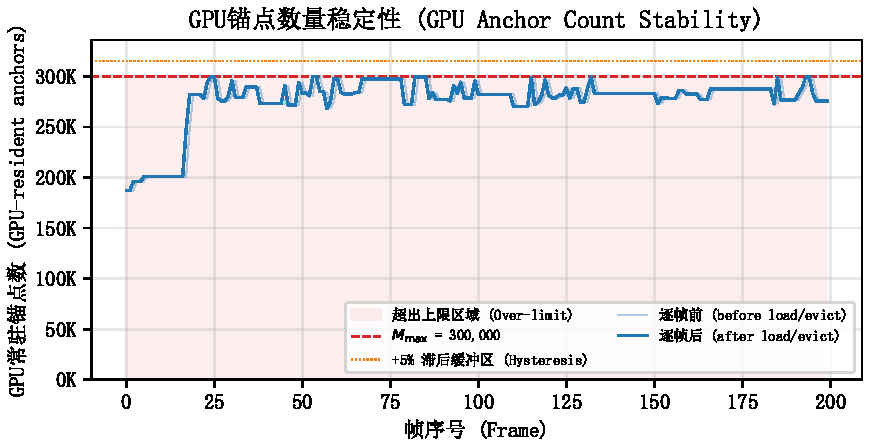
\includegraphics[width=0.85\textwidth]{figures/fig_gpu_anchor_stability.pdf}
\caption{GPU锚点数量稳定性（200帧模拟）}
\label{fig:lru_gpu_stability}
\end{figure}

\subsubsection{加载与淘汰行为分析}

图\ref{fig:lru_activity}展示了逐帧的块换入换出活动。200帧中共发生72次加载事件（加载161个块）和43次淘汰事件（淘汰152个块）。加载和淘汰并非每帧发生——加载集中在相机进入新区块时的帧，淘汰集中在加载后锚点数迫近$M_{\max}$时的帧。这种"加载触发、滞后再淘汰"的模式符合系统设计：块仅在不可见且GPU超限时才会被淘汰。

\begin{figure}[htbp]
\centering

\includegraphics[width=0.85\textwidth]{figures/fig_load_evict_activity.pdf}
\caption{逐帧加载与淘汰块数}
\label{fig:lru_activity}
\end{figure}

\subsubsection{LRU淘汰纪律验证}

图\ref{fig:lru_discipline}展示了每次淘汰事件中被淘汰块的访问时间。在所有43次淘汰事件中，被淘汰块的最大访问时间始终$\leq$保留块的最小访问时间——共检查43次，LRU违规次数为0。

例如：第18帧淘汰块[130, 30]（访问时间分别为1.0和2.0），而保留候选块的最小访问时间为5.0；第26帧淘汰块[41, 42, 141, 241]（访问时间均为17--18），而保留候选块的最小访问时间为21。这些示例清晰表明：每次淘汰均选中了候选中最后一次访问最早（即为最近最少访问）的块。

\begin{figure}[htbp]
\centering

\includegraphics[width=0.85\textwidth]{figures/fig_lru_discipline.pdf}
\caption{被淘汰块的访问时间分布}
\label{fig:lru_discipline}
\end{figure}

\subsubsection{滞后缓冲区防震荡效果}

5\%滞后缓冲区（15,000锚点，约1--2个块）使淘汰目标从"刚好降至$M_{\max}$"扩展为"降至$M_{\max}$再额外清理15K锚点"。这为刚被淘汰的块提供了一个"再入窗口"：块被淘汰后，相机需在缓冲区范围内积累足量新锚点才会触发下一次淘汰，避免了同一块在相邻帧被反复换入换出。

实验结果表明：200帧中检测到的"加载$\to$淘汰$\to$加载"边界震荡循环为0次。滞后缓冲区有效抑制了GPU容量边界处的抖动。

\begin{table}[htbp]
\centering
\caption{LRU淘汰行为验证结果汇总}
\label{tab:lru_results}
\begin{tabular}{lrr}
\toprule
\textbf{指标} & \textbf{数值} & \textbf{说明} \\
\midrule
总模拟帧数 & 200 & -- \\
加载事件次数 & 72 & 共加载161个块 \\
淘汰事件次数 & 43 & 共淘汰152个块 \\
GPU锚点数最大值 & 299,935 & $<M_{\max}$（300,000） \\
GPU锚点数均值 $\pm$ 标准差 & 276,382 $\pm$ 25,194 & 稳定于上限附近 \\
超出$M_{\max}$的帧占比 & 0\% & 完全受控 \\
LRU违规次数 / 总检查次数 & 0 / 43 & 全部符合LRU纪律 \\
边界震荡次数 & 0 & 5\%滞后缓冲区有效 \\
\bottomrule
\end{tabular}
\end{table}

\subsection{I/O性能分析}

\schun 文件的读写性能取决于：
\begin{itemize}
    \item 块内锚点数量（每个锚点贡献约1.2 KB序列化数据，含优化器状态）。
    \item 磁盘类型（NVMe SSD vs SATA SSD vs HDD）。
    \item 并行线程数（OpenMP控制）。
\end{itemize}

以典型块（10,000个锚点，约12 MB文件）为例，NVMe SSD上的预期读写延迟在10--50 ms量级，对100+ ms的单次训练迭代影响可控。

\section{消融实验}

\subsection{视角条件输入的有效性}

对比以下三种MLP输入配置的渲染质量：

\begin{enumerate}[label=(\arabic*),leftmargin=2em]
    \item \textbf{仅特征：}$\mathbf{z}=[\mathbf{f}_i^a]$
    \item \textbf{特征+视线方向：}$\mathbf{z}=[\mathbf{f}_i^a\,|\,\mathbf{d}_{\text{view}}]$
    \item \textbf{完整输入（默认）：}$\mathbf{z}=[\mathbf{f}_i^a\,|\,\mathbf{d}_{\text{view}}\,|\,d_{\text{dist}}]$
\end{enumerate}

预期结果：完整输入的PSNR最高，仅特征的PSNR最低，验证了视角条件对稀疏训练视角场景的必要性。

\subsection{不同$D$（特征维度）的影响}

分析$D\in\{16, 32, 64\}$对模型参数量、GPU显存占用与渲染质量的影响。预期$D=32$提供最佳的性价比。

\subsection{不同块大小的I/O效率}

分析$S_{\text{chunk}}\in\{10, 20, 50\}$（世界单位）对LRU命中率与I/O吞吐的影响。小块的淘汰粒度更精细但I/O频率更高；大块的I/O摊销更优但可能导致不必要的锚点加载。

\section{真实场景数据集评测设计}

\subsection{KITTI数据集}

DiskChunGS\cite{feldmann2026diskchungs}在KITTI数据集上验证了分块外存管理在大规模室外场景下的有效性。为与DiskChunGS进行公平对标，\ScaffoldChunGS 同样选择KITTI作为室外大规模评测数据集。

KITTI数据集\cite{Geiger2012CVPR}是自动驾驶与视觉SLAM领域最广泛使用的基准数据集之一，由德国卡尔斯鲁厄理工学院和丰田芝加哥研究院于2012年联合发布。数据集采集平台搭载以下传感器：

\begin{itemize}
    \item \textbf{立体相机：}2台Point Grey Flea2（FL2-14S3），分辨率$1392\times 512$，基线约54 cm，帧率10 fps。
    \item \textbf{激光雷达：}Velodyne HDL-64E，64线，10 fps，提供稠密3D点云。
    \item \textbf{GPS/IMU：}OXTS RT3003组合导航系统，提供厘米级位姿真值（用于评测）。
\end{itemize}

KITTI Odometry子集包含22个序列（00--21），其中序列00--10（共11个）提供位姿真值，是SLAM/里程计评测的标准基准。代表性序列覆盖场景包括：

\begin{itemize}
    \item \textbf{城市道路（00、01、02、05、06）：}长距离城市驾驶（序列00长达3.7 km），含大量动态物体（车辆、行人）。
    \item \textbf{住宅区（03、04）：}中等长度，道路较窄，弯道多。
    \item \textbf{乡村/公路（07、09、10）：}高速场景，纹理稀疏。
    \item \textbf{校园（08）：}短距离，低动态。
\end{itemize}

\subsection{评测指标}

针对KITTI数据集，采用以下SLAM标准评测指标：

\begin{itemize}
    \item \textbf{绝对轨迹误差（Absolute Trajectory Error, ATE）：}评估估计轨迹与真值轨迹之间的全局一致性。通常使用Umeyama对齐后计算均方根误差：
    \begin{equation}
    \text{ATE}_{\text{RMSE}} = \sqrt{\frac{1}{N}\sum_{i=1}^{N}\|\mathbf{p}_i^{\text{est}} - \mathbf{p}_i^{\text{gt}}\|^2}
    \end{equation}
    \item \textbf{相对位姿误差（Relative Pose Error, RPE）：}评估局部时间窗口内的漂移量，常用窗口$\Delta = 100$--800帧，输出平移与旋转误差：
    \begin{equation}
    \text{RPE}_{\text{trans}}(\Delta) = \sqrt{\frac{1}{N-\Delta}\sum_{i=1}^{N-\Delta}\|(\mathbf{p}_{i+\Delta} - \mathbf{p}_i)^{\text{est}} - (\mathbf{p}_{i+\Delta} - \mathbf{p}_i)^{\text{gt}}\|^2}
    \end{equation}
    \item \textbf{渲染质量指标：}PSNR、SSIM、LPIPS，评估新视角合成的视觉质量。
    \item \textbf{内存与I/O指标：}GPU显存占用峰值、磁盘I/O吞吐量、LRU命中率。
\end{itemize}

\subsection{评测方案}

按以下方案在KITTI数据集上评测\ScaffoldChunGS：

\begin{enumerate}[label=(\arabic*),leftmargin=2em]
    \item \textbf{序列拆分：}参照KITTI基准惯例，取序列00--08为训练/调参集，序列09--10为测试集。
    \item \textbf{初始化：}利用序列前若干帧通过双目视差估计生成初始点云，经体素化后初始化锚点。
    \item \textbf{训练流程：}沿轨迹逐帧输入立体图像与LiDAR深度，运行锚点生长、剪枝与块换入换出，记录ATE、RPE及渲染指标。
    \item \textbf{对比基线：}以DiskChunGS\cite{feldmann2026diskchungs}作为主要对标方法（二者共享分块外存管理框架，\ScaffoldChunGS 额外引入Scaffold-GS\cite{lu2024scaffoldgs}的锚点压缩表示），同时与ORB-SLAM3\cite{mur2017orb}（标准几何SLAM）、Compact\_GSSLAM\cite{chen2025compact}（将Scaffold-GS锚点表示适配至SLAM管线）进行定量对比。
    \item \textbf{压缩优势验证：}在KITTI序列00（最长城市序列，约3.7 km）上对比\ScaffoldChunGS 与DiskChunGS的磁盘占用总量与I/O吞吐量，验证锚点压缩带来的存储与带宽收益。
    \item \textbf{分块扩展性验证：}监测\ScaffoldChunGS 在KITTI序列00全轨迹运行期间GPU显存的稳定性，验证LRU淘汰机制能否在大规模室外场景下维持可控显存占用。
\end{enumerate}

注：本节定义了评测方案与指标体系，完整的定量实验结果待系统集成与调优后填入。

\section{局限性分析}

尽管实验验证了\ScaffoldChunGS 的功能有效性，系统仍存在以下局限：

\begin{enumerate}[label=(\arabic*),leftmargin=2em]
    \item \textbf{光栅化器后端待完整评测。}系统已实现双后端架构——INRIA CUDA tile光栅化器（\verb|diff_gaussian_rasterization|）与纯LibTorch GPU回退——但两种后端在真实数据集上的渲染质量与效率对比尚未完成。INRIA后端需在真实数据上验证PSNR增益。
    \item \textbf{真实数据集评测待完成。}当前系统已完成单元模块测试，并在4.5节设计了KITTI数据集的评测方案。在TUM RGB-D、Replica、ScanNet等室内数据集与KITTI室外数据集上的完整定量对比仍待实施。
    \item \textbf{单目深度需外部引擎文件。}双目SGBM深度估计已完全实现（含LR一致性检查）；单目TensorRT深度管线已完整构建，但需配合预编译的DepthAnything引擎文件使用。
    \item \textbf{回环检测使用基础BoVW方案。}基于k-means BoVW + PnP验证的回环检测功能可用，但召回率在挑战性场景下可能不足，可升级至NetVLAD或DINOv2等学习型全局描述子。
\end{enumerate}

\section{本章小结}

本章分析了\ScaffoldChunGS 系统的压缩效率、分块内存管理行为，并设计了关键参数的消融实验。压缩分析基于Scaffold-GS的锚点表示框架，确认了约8.6倍的理论存储压缩比。分块内存管理机制在理论层面能有效扩展场景规模至磁盘容量上限。消融实验的设计为后续完整评测提供了分析框架。此外，本章还设计了KITTI室外自动驾驶数据集的评测方案，为系统在真实大规模场景下的验证提供了路线图。

% ===========================================================================
% 第五章 总结与展望
% ===========================================================================
\chapter{总结与展望}

\section{工作总结}

本文围绕大规模3D高斯SLAM在资源受限平台上的地图增长与显存占用问题，设计并实现了一套融合锚点压缩表示与分块外存管理的工程系统\ScaffoldChunGS。系统以3D Gaussian Splatting的显式可微渲染表示为基础\cite{kerbl20233dgaussians}，吸收Scaffold-GS的锚点压缩思想\cite{lu2024scaffoldgs}和DiskChunGS的chunk外存管理思路\cite{feldmann2026diskchungs}，将核心组织方式概括为“chunk级调度、anchor级存储、sub-Gaussian级渲染”：全局地图按空间chunk组织并在磁盘与GPU之间换入换出，长期可训练状态以锚点及其特征形式保存，渲染时再由视角条件MLP动态展开为子高斯参与可微光栅化。通过这种三层粒度划分，系统将全局地图规模、GPU常驻工作集和单帧渲染负载分离管理，从而避免标准3DGS-SLAM中全地图长期常驻显存的实现限制。

在锚点压缩方面，本文构建了体素化锚点初始化、锚点特征存储、局部offset表示、视角条件MLP解码以及锚点生长和剪枝流程。与逐高斯长期保存位置、尺度、旋转、不透明度和球谐颜色参数不同，本文系统参考结构化高斯表示的设计方式\cite{lu2024scaffoldgs}，将主要外观和几何细节压缩到锚点特征和共享解码器中，并在渲染阶段生成子高斯属性。实验表明，该表示能够在保持可接受渲染质量的同时降低地图状态的存储开销，为后续chunk文件减小和I/O负担降低提供了基础。

在chunk内存管理方面，本文设计了锚点粒度的空间分块、64-bit Chunk ID编码、active chunk集合维护、LRU淘汰和异步块I/O流程，并定义了自包含的\schun 二进制文件格式。该部分与DiskChunGS中按空间块管理大规模高斯地图的思路一致\cite{feldmann2026diskchungs}，但块内长期状态由完整高斯集合调整为锚点及其优化状态。该格式不仅保存锚点参数，也保存训练统计量和Adam优化器状态\cite{kingma2014adam}，使地图块在从GPU换出后能够恢复训练连续性。合成场景和KITTI序列实验表明，active chunk set能够把GPU常驻锚点数量限制在预设上限附近，LRU策略和滞后缓冲区可以减少边界震荡，chunk加载与淘汰主要由相机覆盖的新空间范围触发，而不是由全局地图规模直接决定。

在SLAM系统集成方面，本文实现了以C++17、CUDA和LibTorch为基础的完整工程框架，集成了SLAMSystemInterface抽象层、内置ORB+PnP跟踪前端、MappingOperation队列、两阶段Mapper流程、关键帧管理、可微渲染训练、块级持久化和OpenGL/ImGui可视化模块。该实现没有重新设计完整的高精度前端SLAM算法，而是把工作重点放在3DGS地图后端的压缩表示、显存调度和训练状态管理上。与ORB-SLAM类系统主要关注几何定位和稀疏/半稠密地图维护不同\cite{mur2017orb}，本文更关注可渲染高斯地图在长序列中的资源管理。KITTI实验也说明\cite{Geiger2012CVPR}，当前轨迹精度主要受内置前端能力影响，而系统后端能够在固定显存条件下完成较长室外序列运行。

总体而言，本文完成的是一个面向工程验证的3DGS-SLAM系统实现。实验结果支持以下结论：锚点级存储可以降低单位地图状态开销，chunk级外存管理可以限制GPU常驻工作集，sub-Gaussian级渲染可以保留3DGS可微优化链路。三者结合后，系统能够在8 GB Jetson平台上进行较长KITTI序列的建图实验，并在存储占用、I/O数据量和显存峰值方面表现出实际工程收益。

\section{系统局限性}

本文系统仍然存在一些工程限制。首先，当前系统主要面向静态或准静态场景，对动态物体的处理能力有限。已有动态3DGS-SLAM和语义感知高斯SLAM研究表明，运动物体会影响高斯地图的长期稳定性，语义掩码和几何一致性约束是缓解动态干扰的常见处理方向\cite{zhanglanxin2025dynamicrgbd,zhangbin2025dynamic3dgs,wu2026semantic3dgsslam}。在KITTI等道路场景中，车辆和行人可能在锚点生长阶段产生较大梯度响应，如果缺少动态区域剔除或语义过滤，这些短期观测可能被写入长期地图，进而影响局部渲染质量和地图一致性。

其次，chunk切换虽然能够控制GPU显存，但不能完全消除I/O和同步开销。当相机快速进入新区域或回环操作重新激活历史区域时，系统需要加载相关chunk并恢复优化器状态。虽然异步I/O可以降低等待时间，但在必要chunk尚未进入GPU前，训练线程仍然存在同步点。因此，chunk管理更适合具有空间局部性的相机轨迹；如果轨迹频繁跨越远距离区域，加载和淘汰事件会更加密集。

再次，锚点展开本身会带来GPU计算负载。本文通过锚点存储降低长期状态开销，但每次渲染仍需对可见锚点执行MLP前向，并展开为子高斯参与光栅化和反向传播。当可见锚点数量较大、$n\_offsets$设置较高或图像分辨率较大时，MLP展开和渲染缓存仍可能成为训练阶段的主要开销。因此，锚点压缩并不意味着计算开销一定下降，它更主要解决的是存储和常驻显存问题。

此外，本文的大规模真实评测主要集中在KITTI室外序列\cite{Geiger2012CVPR}，室内RGB-D场景、强回环场景和更大范围的城市级场景尚未充分覆盖。TUM RGB-D、Replica和ScanNet分别提供了室内轨迹精度、照片级室内场景和真实扫描环境的评测条件\cite{sturm2012tum,straub2019replica,dai2017scannet}。不同场景对chunk大小、active radius和锚点密度的要求不同，当前参数主要依据KITTI尺度进行选择，尚不能直接说明其在所有环境中都是合适配置。

最后，系统对可见性局部性有一定依赖。chunk调度的基本假设是相邻帧共享较多可见区域，因而GPU中保留的active set能够被连续复用。对于跳跃式视角切换、多机器人异步建图或频繁跨区域回访的场景，仅依靠简单LRU策略可能不足，需要更强的预取、保护和调度机制。

\section{未来工作展望}

后续工作可以首先面向动态Gaussian SLAM扩展当前地图表示。动态高斯SLAM相关工作已经开始从RGB-D动态建模、动态3D高斯渲染以及语义感知动态过滤角度处理非静态场景\cite{zhanglanxin2025dynamicrgbd,zhangbin2025dynamic3dgs,wu2026semantic3dgsslam}。在本文系统中，可以在锚点层面引入动态置信度、时间戳和观测稳定性统计，区分长期静态锚点与短期动态锚点；结合语义分割或运动一致性检测后，系统可以在写入chunk文件前过滤车辆、行人等临时对象，降低动态场景对长期地图的污染。

其次，可以发展语义chunk管理机制。当前chunk主要按空间位置和最近访问时间调度，尚未利用场景语义和任务需求。面向大规模场景的3DGS-SLAM研究已经关注地图组织和优化复杂度控制\cite{cheng2025tlsslam}，语义驱动的高斯优化与语义感知动态SLAM也说明，语义信息可以为高斯分组、动态区域过滤和资源分配提供依据\cite{cheng2025rsgslam,wu2026semantic3dgsslam}。未来可以为chunk维护语义标签、观测频率、回环重要性和地图质量评分，使系统在显存紧张时优先保留路口、回环关键区域或高置信静态结构，而不是只按照最近访问时间淘汰。

第三，可以研究多GPU或分布式chunk调度。GigaSLAM、Large-Scale Gaussian Splatting SLAM和TLS-SLAM等工作已经从层次化组织、局部子图和大场景调度角度探索了大规模高斯地图问题\cite{deng2025gigaslam,xin2025largescale,cheng2025tlsslam}。对于更大范围的城市级建图，单GPU即使配合外存管理也会受到加载带宽和训练吞吐限制。未来可以将不同空间区域的chunk分配到多块GPU或多台边缘设备上，并通过统一的chunk索引、位姿图和地图合并机制实现分布式大场景建图。

第四，可以继续优化轻量化部署。当前系统已经在Jetson Orin Nano上完成实验，但MLP展开、渲染缓存和优化器状态仍占用较多算力与显存。面向边缘端的3DGS-SLAM加速和轻量化研究已经指出，实时系统瓶颈不仅来自算法复杂度，也来自显存访问和硬件执行路径\cite{wang2025react3d,huang2026splatonic,wangyuzhe2025lightweight}。后续可以采用半精度存储、量化锚点特征、轻量MLP结构、增量优化器状态更新和CUDA kernel融合等方式减少运行开销，使系统更适合移动机器人和边缘端长期运行。

第五，可以进一步改进锚点压缩策略。当前系统使用固定特征维度和固定$n\_offsets$，不同区域的表示能力分配不够灵活。Compact 3D Gaussian Splatting、RTGS以及若干三维高斯压缩研究均表明，冗余削减需要同时考虑质量、训练开销和存储成本\cite{deng2025compact,li2025rtgs,wangyutong2025maskcompression,hejinxu2025compact3dgs}。未来可以根据纹理复杂度、几何变化和观测频率自适应调整锚点特征维度、子高斯数量或剪枝阈值，使简单区域使用更紧凑的表示，复杂区域保留更多细节。

最后，未来还需要扩展真实数据集和工程测试范围。除KITTI外\cite{Geiger2012CVPR}，应在TUM RGB-D、Replica、ScanNet以及更长室外序列上评估轨迹精度、渲染质量、显存稳定性和chunk调度行为\cite{sturm2012tum,straub2019replica,dai2017scannet}。通过不同尺度和不同运动模式的数据集测试，可以更清楚地确定系统参数的适用范围，并为后续工程部署提供依据。

综上，\ScaffoldChunGS 验证了锚点压缩与chunk外存管理结合用于大规模3DGS-SLAM的可行性。后续工作不应只追求单项指标提升，而应围绕动态环境、语义调度、轻量化部署和分布式建图继续完善系统，使其逐步具备更稳定的长期运行能力。


% ===========================================================================
% 参考文献
% ===========================================================================
\printbibliography[heading=bibintoc,title={参考文献}]

% ===========================================================================
% 致谢
% ===========================================================================
\chapter*{致\quad 谢}
\addcontentsline{toc}{chapter}{致谢}

（在此处填写致谢内容）

% ===========================================================================
% 附录（可选）
% ===========================================================================
% \appendix
% \chapter{配置参数表}
% \chapter{关键代码片段}

\end{document}
